\documentclass[conference]{IEEEtran}
%\IEEEoverridecommandlockouts
% The preceding line is only needed to identify funding in the first footnote. If that is unneeded, please comment it out.
\usepackage{cite}
\usepackage{amsmath,amssymb,amsfonts}
\usepackage{algorithm}
\usepackage{algorithmic}
\usepackage{graphicx}
\usepackage{textcomp}
\usepackage{listings}
\usepackage{fancyvrb}
\usepackage{xcolor}
\usepackage[makeroom]{cancel}
\def\BibTeX{{\rm B\kern-.05em{\sc i\kern-.025em b}\kern-.08em
    T\kern-.1667em\lower.7ex\hbox{E}\kern-.125emX}}
\begin{document}

\title{Adapting VBASBS Queueing Model for Proof-of-Stake Consensus Algorithm}

\author{
  \textbf{Kyle Kentner$^*$, Nathan Crosby$^*$, Andrew Smith$^*$, Sush Chittibabu$^*$, and Abdulla Karjikar$^*$}\\
  Oklahoma State University - Stillwater, OK \\
  kyle.kentner@okstate.edu, ncrosby@okstate.edu, scu@okstate.edu, \\
  sushmitha.chittibabu@okstate.edu, abdulla.karjikar@okstate.edu}

\maketitle

\def\thefootnote{*}\footnotetext{These authors contributed equally to this work, but the group member Rohith Alamuri did not contribute to this paper.}\def\thefootnote{\arabic{footnote}}

\begin{abstract}

Our main goal with this work is to establish a theoretical model that can simulate
more accurately how blockchain transactions are grouped, validated, processed,
and purged from a network based on a proof-of-stake consensus algorithm. With 
the switch from the proof-of-work consensus algorithm to the newer proof-of-stake with 
cryptocurrencies, most notably Ethereum, there is a need to update the theoretical 
models that are used to define efficiency metrics. Further, we took it upon ourselves 
to move beyond that and quantify the optimal time window to decrease waiting time
for the average owner of each transaction, while not significantly deteriorating throughput
for the network as a whole.

\end{abstract}

\begin{IEEEkeywords}
Blockchain, Optimization, Queueing
\end{IEEEkeywords}

\section{Introduction}\label{Intro}

The blockchain, a distributed ledger utilizing records linked together via cryptographic 
hashes, has within the last decade captivated the industry. Having been utilized in the 
development of a decentralized economic transfer scheme with the adoption of 
Bitcoin\cite{2008_Bitcoin_Nakamoto}, the original proof-of-work concept had established 
a means of validating incoming transactions through a distributed network of participants. 
This led to the development of other crypto-currency applications, most notably Ethereum. 
These solutions implemented methods with a focus on the accuracy and redundancy of the 
various transactions with minimal effort given to reduce individual transactional waiting 
time and increase the efficiency of processing transactions.

This approach remains true for Bitcoin; however, Ethereum changed this consensus 
mechanism in 2022 with the update to proof-of-stake\cite{2022_Ethereum_PoS}. This 
changed the blockchain to be more efficient in reducing complexity in the work 
computations while decreasing the barrier to entry hence providing reduced centralized 
risk with the potential of more nodes securing the network. Where under the proof-of-work
consensus algorithm, the timing of blocks was determined by the mining difficulty, the 
new approach, proof-of-stake, the timing is fixed. Time in the Ethereum proof-of-stake 
consensus algorithm is divided into slots of 12 seconds and epochs of 32 slots.

While the proof-of-stake greatly improved the efficiency of transactions, there remains 
room for improvements in the validation of transactions. In this paper, we propose an 
algorithm to decrease waiting time while maintaining a high level of throughput. To begin 
the optimization process, we must first choose a performance model that analytically 
describes the relationship between the number of transactions, the fixed time for those 
transactions to be processed, and the total number of transactions that are processed 
(throughput). Once a representative performance model has been chosen, an optimal
time window can be selected that balances out the throughput. 

Our paper is organized as follows. In section two we conduct a brief literature review and 
then focus on the performance model that will underly our own work. Section three is 
dedicated to the methodology we used to optimize the block size with details of our 
approach theorized via mathematical models. In section four, we discuss the results recorded 
from our early attempts at simulating our proposed model. Then we conclude in section five 
with remarks and discuss potential future areas to continue expanding upon the model. 

\section{Related Work}\label{related}

One of the main detriments of the concept of cryptocurrencies has been the slow transaction
rates with proof-of-work consensus algorithm validation of transactions. The main focus to rectify 
this problem while maintaining the original consensus algorithm can be seen in previous work such 
as Fu\cite{2020_IEEEToVT_Fu}. This work states that when considering blockchain optimization, 
the throughput, or number of transactions processed by a blockchain system in a given amount of 
time, are key indicators of its performance. Mechkaroska\cite{2018_TELFOR_Mechkaroska} explores
some of the methods tried up to that point. They include increasing the block size to increase the 
number of transactions being processed, which is increasing throughput, and a technique called 
"sharding" that is similar to parallel processing of transactions. This showed up in an alt-coin named 
Zilliqa\cite{2017_Zilliqa_Zilliqa} which is mentioned in the paper. While sharding is on the docket of 
potential changes to the Ethereum network, it has not been given the green light yet, and might not
be necessary considering the changes made to the consensus algorithm, discussed later.

The prevalence of articles that called for an increase to the block size to a na\"ive larger size shows 
a lack of creativity to solve this issue of slow transaction validation as can be seen in Gobel, Thakkar, 
and Mechkaroska\cite{2017_IEEE_Gobel, 2018_IEEE_Thakkar, 2018_TELFOR_Mechkaroska}. The 
hard fork in Bitcoin to create Bitcoin Cash was chiefly designed to make this change, with the increase 
in block size from 1MB on Bitcoin to 8MB on Bitcoin Cash. 

\begin{figure*}[htbp]
    \centerline{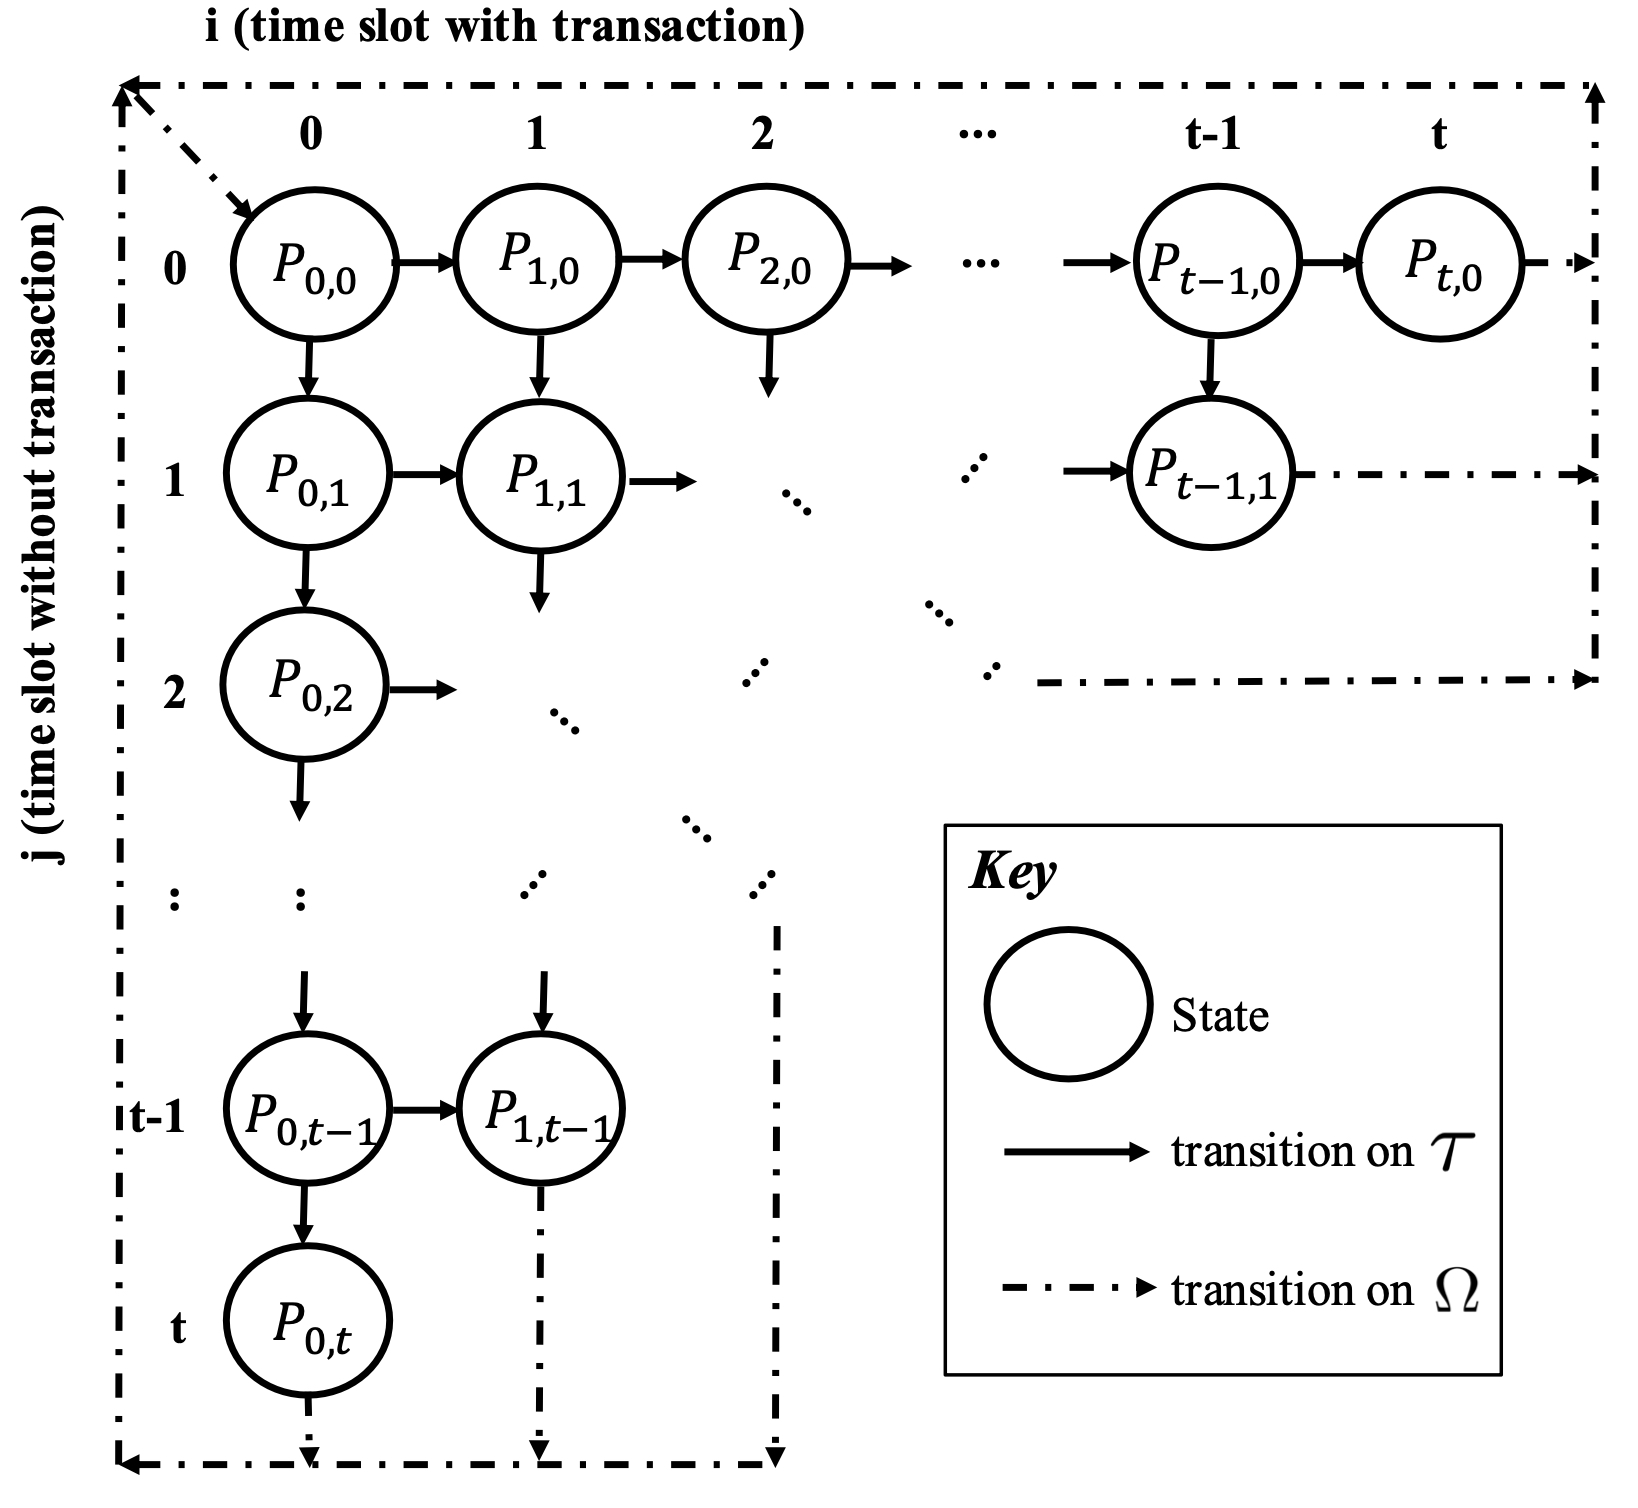
\includegraphics[width=\textwidth]{Figures/Flow}}
    \caption{State transition diagram of new model.} 
    \label{flow}
\end{figure*}	

Proof-of-work consensus algorithms take such a long time to calculate as a safety precaution against
Sybil attacks. This methodology is no longer required for large market cap cryptocurrencies, and a 
shift to a proof-of-stake consensus algorithm facilitates a precipitous drop in energy consumption
as seen in Platt\cite{2021_IEEEQRSC_Platt}. The large pool of staked validators means that the 
requirement for a validator can switch from access to raw compute power to capital. As stated in 
Sec.~\ref{Intro} this change for Ethereum happened in 2022, and therefore a new theoretical model
must be considered to take into account the eccentricities of this new consensus algorithm. 

\section{Methodology}

\subsection{Original Performance Model}\label{Model}
Our algorithm will expand on the performance model proposed by Seol, Kancharla, Ke, Kim and Park
 - A Variable Bulk Arrival and Static Bulk Service Queuing Model for Blockchain\cite{2020_ACM_Seol}. 
 In the initial model, the arrival rate of the individual blockchain transactions is variable, but not unpredictable. 
 The arrival rate is assumed to vary with the size of the incoming transaction and the rate is 
 denoted by the symbol $\lambda$.

The variable $\mu$ is defined to be the processing time of a block to be posted and purged as noted 
in Seol\cite{2020_ACM_Seol}, and is assumed to be fairly static as stated in the model. 
The variable n is defined to be the total number of slots in the block. P$_i$ denotes the states with 
P$_n$ denoting the maximum state before the block is processed. 

This model was based off of a proof-of-work concept as can primarily be seen with cryptocurrencies 
such as Bitcoin, as stated in Sec.~\ref{Intro}. The crux of the argument for this balance set of equations 
lies in Eq. 1 in Seol\cite{2020_ACM_Seol}, and also here, and thus will be the basis for our 
new model. 

\begin{equation}
P_n = \frac{\lambda}{\mu}\frac{n(n+1)}{2}P_0\label{om_1}
\end{equation}

\subsection{New Performance Model}\label{new_model}

Due to the Ethereum network switching from the proof-of-work to proof-of-stake 
concept for their consensus algorithm, as discussed in Sec. ~\ref{related}, we have 
decided to update the base model in Seol\cite{2020_ACM_Seol} to reflect this new 
regime. This new proof-of-stake methodology essentially flips the previous base 
model on its head, where the time between blocks being pushed out to validators is 
set at a fixed interval, and because of this, the block size can then fluctuate based 
on the number of transactions that have arrived in the latest block window of time. 
To account for this we have discretized the block time window into single transaction
slots based on the theoretical maximum number of transactions that can arrive on 
the network per second. In each slot we can then either have a transaction arrive, 
or not. 

The subsequently updated variables and assumptions are given below. 

$P_{0,0}$: The state at which no time has passed in the block window of time ($T$). 

$P_{t,0}$: The state at all of the time has passed in the block window of time ($T$), and
the block is ready to be sent to the validator community, with no empty time slices, so 
$n = t$. 

$P_{t-j,j}$: The state where all of the time has passed in the block window of time ($T$), and
the block is ready to be sent to the validator community, with $j$ empty time slices. 

$P_{i,0}$: The state at which $i$ transactions have arrived in the 
block window of time with 0 empty time slices. 

$P_{i,j}$: The state at which $i$ transactions have arrived in the 
block window of time with $j$ empty time slices. 

$\tau$: The minimum time increment that can pass between the 
transaction arrivals. If the theoretical maximum for a given application is 1,000 transactions 
per second then $\tau = \frac{1}{1000}$

$T$: The total time that will pass between each block creation and is initially static.

$t$: The total number of transactions that can be seen in one block window of time.
This is calculated as $\frac{T}{\tau}$, therefore if $T$ is fixed at twelve seconds and
$\tau=\frac{1}{1000}$ then $t=\frac{12}{\frac{1}{1000}}=12,000$. 

$\Omega$: The rate for the entire block to be posted and purged. This is assumed
to balance the new form of equations as $\mu$ did in the original base model.

$n$: The number of transactions in the block. This is now dependent on $j$ which is
the number of empty time slices that has been seen in the current block window. Here, 
$n=t - j$ or the total possible transactions, minus the empty time slices seen in the
block window of time

\subsubsection{$P_{0,0}$}

The initial state must be set up based on the state transition diagram given in Fig.~\ref{flow}.
Based on that diagram the incoming and outgoing transitions are given below which yields the 
balanced equation in Eq.~\ref{nm_1}. As can be seen, at each time step there is a binary 
observation of either seeing a transaction or not, which equates to either incrementing $i$ by
one or $j$ by one. $\\$

\begin{figure}[htbp]
    \centerline{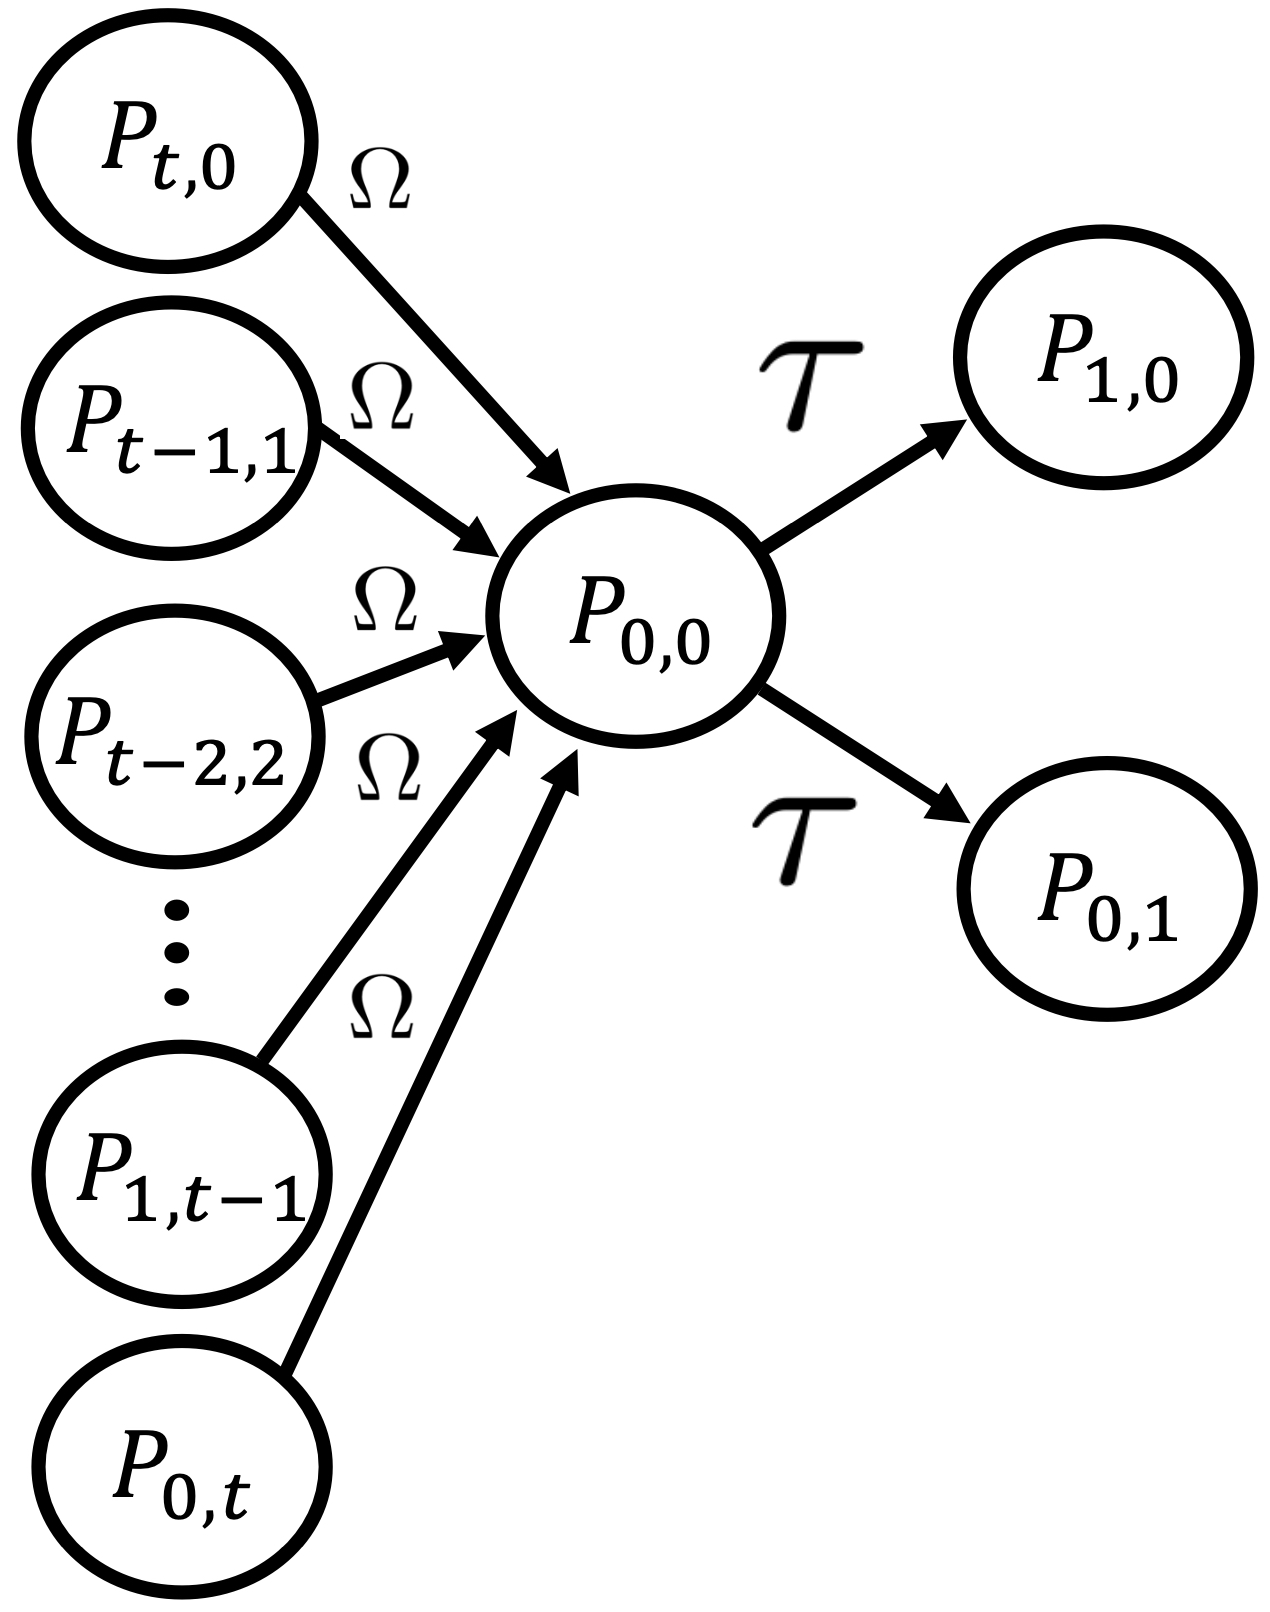
\includegraphics[width=\linewidth]{Figures/P_0,0}}
    \caption{State Transition Diagram of $P_{0,0}$} 
    \label{P_0,0}
\end{figure}	

Incoming: $\Omega (P_{t,0}, P_{t-1,1}, ... , P_{1,t-1}, P_{0,t})$

Outgoing: $2 \tau P_{0,0}$

\begin{equation}
  \Omega(P_{t,0} + P_{t-1,1} +  ... + P_{1,t-1} + P_{0,t})= 2\tau P_{0,0}\label{nm_1}
\end{equation}

To simplify this equation to solve for $P_{0,0}$ we can sum the ending states and
divide both sides by $2\tau$ to end up with Eq.~\ref{nm_2}.

\begin{equation}
  P_{0,0} = \frac{\Omega}{2\tau}\sum_{j=0}^{t}{P_{t-j,j}}\label{nm_2}
\end{equation}

As can be seen here, our new set of equations will be based on time instead of 
a set number of transactions filling up a block. Our newly added parameter $j$ for 
the time slices without a transaction present are essentially stall cycles waiting 
for the next transaction to arrive and have the effect of splitting the final state, 
$P_t$ from the base model in Seol\cite{2020_ACM_Seol} into various states 
from $0$ empty time slices up to $t$ empty time slices. In the event of $t$ 
empty time slices there would be no transactions to validate, however it would 
still need to be verified by the validator community that indeed no transactions 
had arrived, so the empty block would still need to be sent out. 

It is with this addition, along with chopping a fixed amount of time to minimum time
increments, $\tau$, that we can approximate the proof of stake workflow in 
blockchain networks, like Ethereum. 

\subsubsection{$P_{i,j}$} $\\$

Now that the initial state has been defined, we need to examine how the network
will handle the intermediate time steps before we reach the end of the block window
of time ($T$). At each time step, we only have two options, increment $i$ or increment
$j$ based on seeing a transaction or not. Let's first examine the case of $P_{1,0}$ or 
seeing a transaction in the first time slot. $\\$

\begin{figure}[htbp]
    \centerline{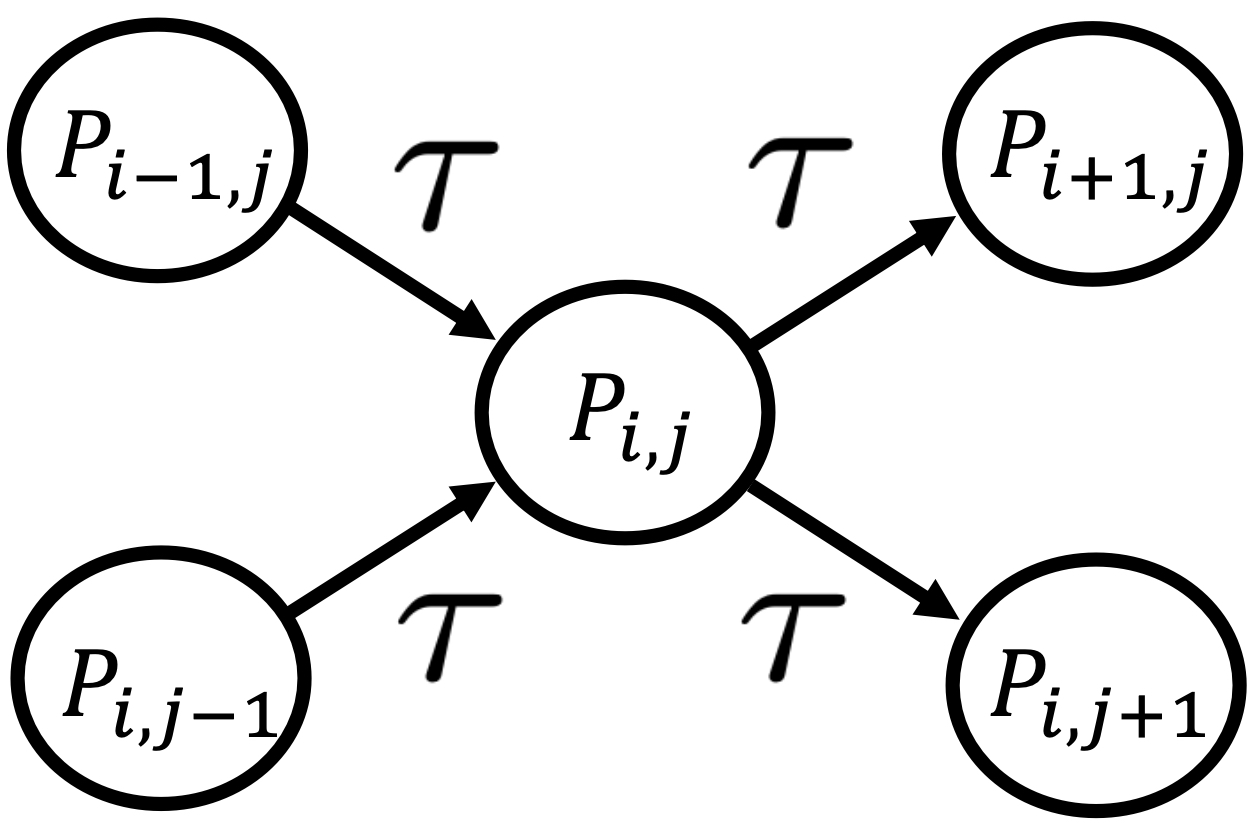
\includegraphics[width=\linewidth]{Figures/P_i,j}}
    \caption{State Transition Diagram of $P_{i,j}$} 
    \label{P_i,j}
\end{figure}

Incoming: $\tau P_{0,0}$

Outgoing: $2 \tau P_{1,0}$

\begin{equation}
  \bcancel{\tau}P_{0,0} = \\
  2\bcancel{\tau}P_{1,0}\label{nm_3}
\end{equation}

\begin{equation}
  P_{1,0} = \frac{1}{2}P_{0,0}\label{nm_4}
\end{equation}

Similarly, we can expand from $P_{0,0}$ to $P_{0,1}$ with Eqs.~\ref{nm_5} \&~\ref{nm_6}

\begin{equation}
  \bcancel{\tau}P_{0,0} = \\
  2\bcancel{\tau}P_{0,1}\label{nm_5}
\end{equation}

\begin{equation}
  P_{0,1} = \frac{1}{2}P_{0,0}\label{nm_6}
\end{equation}

This makes intuitive since, given the binary nature of the observation that after 
one time step and the random nature of $j$ that there is a 50\% chance of landing
in either state $P_{1,0}$ or $P_{0,1}$. We can now move on to the next layer, which 
would then be the states $P_{2,0}$, $P_{0,2}$, or $P_{1,1}$. Lets first examine the 
edge cases. $\\$

Incoming: $\tau P_{1,0}$

Outgoing: $2 \tau P_{2,0}$

\begin{equation}
  \bcancel{\tau} P_{1,0} = 2\bcancel{\tau} P_{2,0}\label{nm_7}
\end{equation}

\begin{equation}
  P_{2,0} = \frac{1}{2}P_{1,0}\label{nm_7}
\end{equation}

And now subbing back into $P_{1,0}$ the result from Eq.~\ref{nm_4} we get:

\begin{equation}
  P_{2,0} = \frac{1}{2}(\frac{1}{2}P_{0,0})=\frac{1}{4}P_{0,0}\label{nm_8}
\end{equation}

And similarly for $P_{0,2}$ we get the same result. Now, lets move on to the more
interesting result from $P_{1,1}$. $\\$

Incoming: $\tau P_{1,0}$, $\tau P_{0,1}$

Outgoing: $2\tau P_{1,1}$

\begin{equation}
  \tau P_{1,0} + \tau P_{0,1} = 2\tau P_{1,1} \label{nm_9}
\end{equation}

\begin{equation}
  \bcancel{\tau} (P_{1,0} + P_{0,1}) = 2\bcancel{\tau} P_{1,1} \label{nm_10}
\end{equation}

\begin{equation}
  P_{1,1} = \frac{1}{2}(P_{1,0} + P_{0,1})\label{nm_11}
\end{equation}

Subbing back in the results for $P_{1,0}$ and $P_{0,1}$ we have:

\begin{equation}
  P_{1,1} = \frac{1}{2}(\frac{1}{2}P_{0,0} + \frac{1}{2}P_{0,0})=\frac{1}{2}P_{0,0}\label{nm_12}
\end{equation}

So, now we have the first two layers and the pattern is starting to emerge, but
let us look at one last layer. The edge cases in the third layer follow the same pattern
as layer two and $P_{3,0}$, and symmetrically $P_{0,3}$, are simply given in Eq.~\ref{nm_13}.

\begin{equation}
  P_{3,0} = P_{0,3} = \frac{1}{8}P_{0,0}\label{nm_13}
\end{equation}

The interesting states here are $P_{2,1}$ and $P_{1, 2}$ derived as follows 
for $P_{2,1}$ and extrapolated to $P_{1,2}$:

\begin{equation}
  \tau P_{1,1} + \tau P_{2,0} = 2\tau P_{2,1} \label{nm_14}
\end{equation}

\begin{equation}
  \bcancel{\tau} (P_{1,1} + P_{2,0}) = 2\bcancel{\tau} P_{2,1} \label{nm_15}
\end{equation}

\begin{equation}
  P_{2,1} = \frac{1}{2}(P_{1,1} + P_{2,0})\label{nm_16}
\end{equation}

Subbing back in for $P_{1,1}$ and $P_{2,0}$ we have:

\begin{equation}
  P_{2,1} = \frac{1}{2}(\frac{1}{2}P_{0,0} + \frac{1}{4}P_{0,0}) = \frac{3}{8}P_{0,0}\label{nm_17}
\end{equation}

And the result from Eq.~\ref{nm_17} is the same for $P_{1,2}$. We can now generalize
for the generic state of $P_{i,j}$. We notice that each layer multiplies the denominator in 
the previous layer by 2, and if we give the denominator the name $b$ then it can be defined
as in Eq.~\ref{nm_18} given that the layer is defined by $i+j$. 

\begin{equation}
  b_{i,j} = 2^{(i+j)}\label{nm_18}
\end{equation}

The numerators will depend on the numerators of the two states that transition to that
state, as long as they are not an edge state (with $i$ or $j$ equal to 0). 

\begin{equation}
  a_{i,j} =
    \begin{cases}
      1,                            & i = 0 \text{ }|\text{ } j = 0 \\
      a_{i-1,j} + a_{i,j-1},  & \text{otherwise}
    \end{cases}
    \label{nm_19}
\end{equation}

Now, the generalized formula for $P_{i,j}$ can be given in Eq.~\ref{nm_20}:

\begin{equation}
  P_{i,j} = \frac{a_{i,j}}{b_{i,j}}P_{0,0}, \text{  for } j < t \text{ \& } i < t-j\label{nm_20}
\end{equation}

\subsubsection{$P_{t-j,j}$} $\\$

We have now defined the initial state, $P_{0,0}$ and the intermediate states, $P_{i,j}$ up 
until we get to the end of the block time window ($T$). We must now define the final states
in our new model. 

\begin{figure}[htbp]
    \centerline{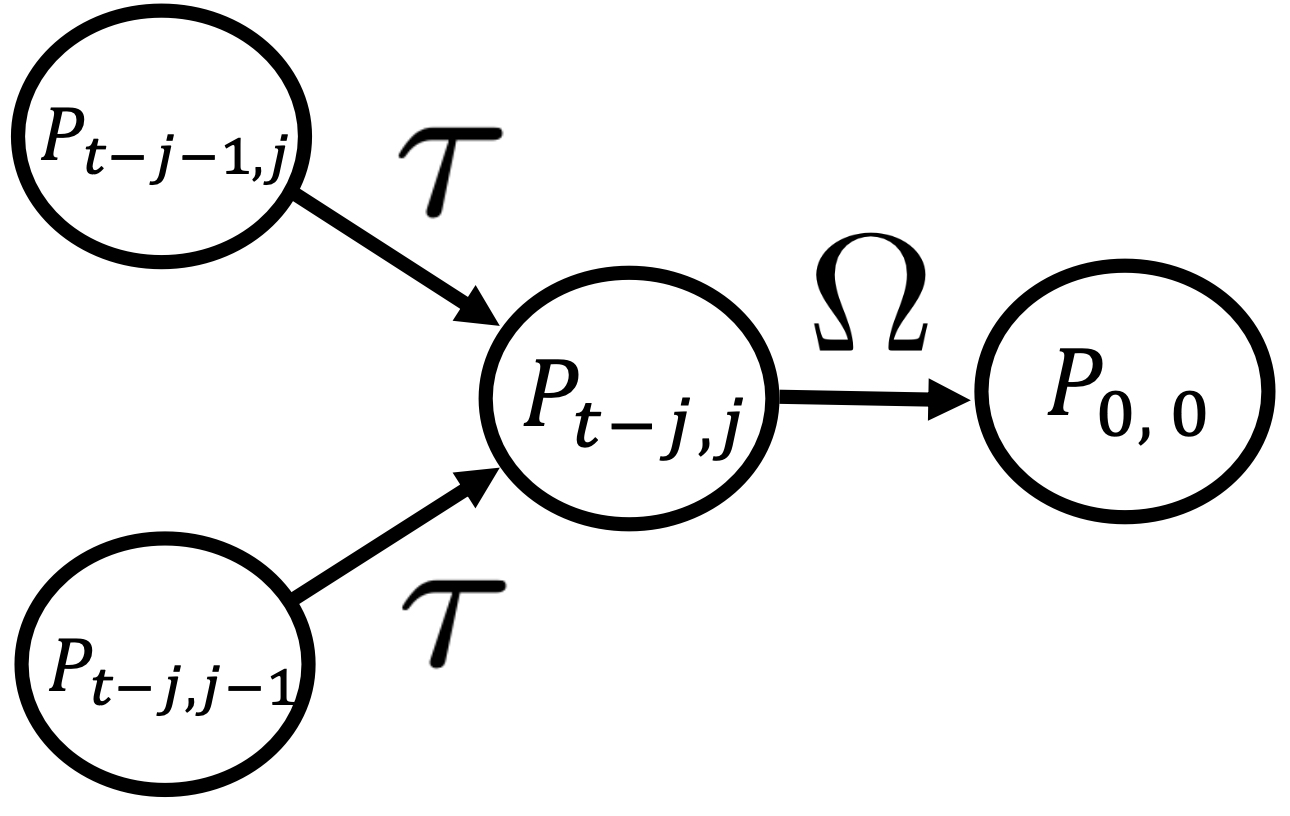
\includegraphics[width=\linewidth]{Figures/P_t-j,j}}
    \caption{State Transition Diagram of $P_{t-j,j}$} 
    \label{P_t-j,j}
\end{figure}

Incoming: $\tau P_{t-j-1,j}$, $\tau P_{t-j,j-1}$

Outgoing: $\Omega P_{t-j,j}$

\begin{equation}
  \tau P_{t-j-1,j} + \tau P_{t-j,j-1} = \Omega P_{t-j,j}\label{nm_21}
\end{equation}

\begin{equation}
  P_{t-j,j} = \frac{\tau}{\Omega} (P_{t-j-1,j} + P_{t-j,j-1})\label{nm_21}
\end{equation}

There are now two cases to consider, the first is when $0<j<t$ and the
other is when $j$ is one of the edge cases. The main caveat is that an 
edge case will have a numerator equal to $1$, where the regular rules
from Eq.~\ref{nm_19} apply to the non-edge cases. Another note, since 
all final states transition to the initial state, $P_{0,0}$, then we do not 
double the numerator again and $b_{t-j,j} = 2^{t-1}$ for all cases. Given 
that, our equations for each final state $P_{t-j,j}$ are as stated in Eq.~\ref{nm_22}.

\begin{equation}
  P_{t-j,j} =
    \begin{cases}
      \frac{a_{t-j-1,j} + a_{t-j,j-1}}{2^{t-1}}P_{0,0},                            & 0 < j < t \\
      \frac{1}{2^{t-1}}P_{0,0},  & j = 0 \text{ } |\text{ } j = t
    \end{cases}
    \label{nm_22}
\end{equation}

\subsubsection{Constraint: Markovian Queueing Assumption}

\begin{equation}
  \sum_{i=0}^{t-j}{\sum_{j=0}^{t}{P_{i,j}}} = 1.0\label{nm_23}
\end{equation}

This can be broken down into the constituent components, starting with the
initial state. The edge cases before the final states are the second unique case
since there coefficients can be calculated as $1/b_{i,j}$ where $b_i,j$ is given in 
Eq.~\ref{nm_18}. The standard $P_{i,j}$ cases come next, followed by the final
states $P_{t-j,j}$. These final states can be further be broken down into there 
middle cases an the two edge cases when $i = 0$ or $j = 0$. 

\begin{multline}
  P_{0,0} +  \sum_{i = 1}^{t-1}{P_{i,0}} + \sum_{j = 1}^{t-1}{P_{0,j}} + \sum_{i=1}^{t-j}{\sum_{j=1}^{t-1}{P_{i,j}}} \\
  + \sum_{j=1}^{t-1}{P_{t-j,j}} + P_{t, 0} + P_{0, t} = 1.0 \label{nm_24}
\end{multline}

Now, all of these cases can be written in terms of $P_{0,0}$ in Eq.~\ref{nm_25} below:

\begin{multline}
  P_{0,0} +  \sum_{i = 1}^{t-1}{\frac{1}{b_{i,0}}P_{0,0}} + \sum_{j = 1}^{t-1}{\frac{1}{b_{0,j}}P_{0,0}} + 
  \sum_{i=1}^{t-j}{\sum_{j=1}^{t-1}{\frac{a_{i,j}}{b_{i,j}}P_{0,0}}} + \\
  \sum_{j=1}^{t-1}{\frac{\tau}{\Omega}\left[\frac{a_{t-j-1,1}}{b_{t-j-1,1}} + \frac{a_{t-j,j-1}}{b_{t-j,j-1}}\right]P_{0,0}} + \\
  \frac{2\tau}{\Omega}\frac{1}{2^{t-1}}P_{0,0} = 1.0 \label{nm_25}
\end{multline}

If we factor out $P_{0,0}$ we get:

\begin{multline}
  P_{0,0} \left[1 +  \sum_{i = 1}^{t-1}{\frac{1}{b_{i,0}}} + \sum_{j = 1}^{t-1}{\frac{1}{b_{0,j}}} + \right.
  \left.\sum_{i=1}^{t-j}{\sum_{j=1}^{t-1}{\frac{a_{i,j}}{b_{i,j}}}} + \right.\\
  \left.\sum_{j=1}^{t-1}{\frac{\tau}{\Omega}\left[\frac{a_{t-j-1,1}}{b_{t-j-1,1}} + \frac{a_{t-j,j-1}}{b_{t-j,j-1}}\right]} + \right.\\
  \left.\frac{\tau}{\Omega}\frac{1}{2^{t-2}}\right] = 1.0 \label{nm_26}
\end{multline}

Finally, if we divide by all of the coefficients then we have our ultimate constraint in Eq.~\ref{nm_27}:

\begin{multline}
  P_{0,0} = \left[1 +  \sum_{i = 1}^{t-1}{\frac{1}{b_{i,0}}} + \sum_{j = 1}^{t-1}{\frac{1}{b_{0,j}}} + \right.
  \left.\sum_{i=1}^{t-j}{\sum_{j=1}^{t-1}{\frac{a_{i,j}}{b_{i,j}}}} + \right.\\
  \left.\frac{\tau}{\Omega}\left(\sum_{j=1}^{t-1}{\left[\frac{a_{t-j-1,1}}{b_{t-j-1,1}} + \frac{a_{t-j,j-1}}{b_{t-j,j-1}}\right]} + \right.\right.
  \left.\left.\frac{1}{2^{t-2}}\right)\right]^{-1} \label{nm_26}
\end{multline}


\subsection{Optimization}\label{optimization}  

Optimization in the old base model pertained to maximizing throughput
while minimizing waiting time by adjusting the size of the next block, $n$,
based on the expected rate of transaction arrivals, $\lambda$. 

Since we have now flipped the model on its head and time is fixed for the next
block sent to validators and the block size already varies, we set out to see if
we can loosen this constraints and set an optimal $T$ based on how fast 
transactions are reaching the network. In our new model, this is entirely based
on $j$ since that variable represents time slices, $\tau$, with no transactions in them,
or as we have also stated, each $j$ can be thought of as a stall cycle waiting for
the next transaction to arrive.

Throughput is then the number of transactions in a given amount of time. 

\begin{equation}
  Throughput = \frac{n}{T}\label{opt_1}
\end{equation}

As is stated in the definitions at the beginning of Sec.~\ref{new_model},
$n=t-j$ and also $t = \frac{T}{\tau}$, so we then have:

\begin{equation}
  Throughput = \frac{\frac{T}{\tau}-j}{T}=\frac{1}{\tau}-\frac{j}{T}\label{opt_2}
\end{equation}

The waiting time for each customer in the queue is now simply $T$

\begin{equation}
  \frac{Throughput}{WaitingTime} = \frac{\frac{1}{\tau}-\frac{j}{T}}{T} = \frac{1}{\tau T}-\frac{j}{T^2}\label{opt_2}
\end{equation}

To find the optimal level of $T$ we then need to take the partial derivative with respect to $T$ that will
be in terms of $j$ and then set it equal to zero and solve for $T$. For simplicity in Eq.~\ref{opt_3}, 
let's call the ratio of Throughput to Waiting Time $M$, and we can calculate the derivative as follows.

\begin{equation}
  \frac{\delta M}{\delta T} = -\frac{1}{\tau T^2}+\frac{2j}{T^3}=0\label{opt_3}
\end{equation}

\begin{equation}
  \frac{1}{\tau T^2}T^3=\frac{2j}{T^3}T^3\label{opt_4}
\end{equation}

\begin{equation}
  T=2j\tau \label{opt_5}
\end{equation}

It is therefore shown that, based on our new model for proof-of-stake networks, the optimal 
time window is two times the number of stall cycles $j$ times the size of the time slice $\tau$.
Since $\tau$ is known and a technical requirement of the network (theoretical max transactions
per second), we only need to estimate $j$ for the coming period to then broadcast the next time 
window $T$ when the previous block is sent out to be validated. For practical purposes, the 
ceiling of the solution to Eq.~\ref{opt_5} should be used to make sure that the time interval is always at least one
second and that there are discrete second intervals to choose from.

\section{Results}

TODO: Redo this later

\section{Conclusion and Discussion}

The conclusion this team has derived through the suggested mathematical models is that 
the blockchain transactions, in regards to proof-of stack, can be optimized in the model 
described in Seol\cite{2020_ACM_Seol}. This is achievable, as suggested in Sec. III, through 
time variable transactions into the queuing model. In this proposed solution, a significant 
reduction is noticeable in transaction waiting time in the queue while maintaining acceptable 
levels of throughput.

Additional research recommended would be to expand this methodology into a future 
Ethereum branch where sharding has been implemented. We believe that this approach, 
along with asynchronous composability inherited from the necessity for the splltting of the 
Ethereum infrastructure, would facilitate optimization on the various transactional validation 
required on such a scale.

\bibliographystyle{IEEEtrans}
\bibliography{Crosby}

\end{document}
